\section*{Metodyka testów}
Efekty treningu sieci zostaną przetestowane na 4 zbiorach danych:
\begin{itemize}
    \setlength\itemsep{-1.5em}
    \item zbiór treningowy MNIST (60000 elementów) - oznaczony $ZT$
    \item zbiór testowy MNIST (10000 elementów) - oznaczony $ZT1$
    \item zbiór testowy stworzony przeze mnie (30 elementów) - oznaczony $ZT2$
    \item zbiór testowy stworzony przez osobę trzecią (30 elementów) - oznaczony $ZT3$
\end{itemize}
Zbiór MNIST został przygotowany w postaci odpowiedniej dla sieci neuronowej, natomiast zbiory $ZT2$ i $ZT3$ muszą zostać odpowiednio zmienione. W wersji podstawowej, dla każdego obrazu został zwiększony kontrast, następnie zmieniono RGB na skalę szarości, oraz zmapowano wartości pixeli na $0$ lub $1$. Finalnie obrazy zostały zeskalowane do rozmiaru 28 x 28. Dodatkowo, dla każdego ze zbiorów $ZT2$ i $ZT3$ został stworzony dodatkowy zbiór (odpowiednio $ZT2\_PREPROCESSED$ i $ZT3\_PREPROCESSED$), który dokładniej przystosował zdjęcia na potrzeby sieci. Z każdego zdjęcia została wycięta część zawierająca cyfrę, następne zeskalowana do 20px, oraz wstawiona w obraz 28 x 28.

\begin{figure}[!htb]
\minipage{0.32\textwidth}
    \centering
    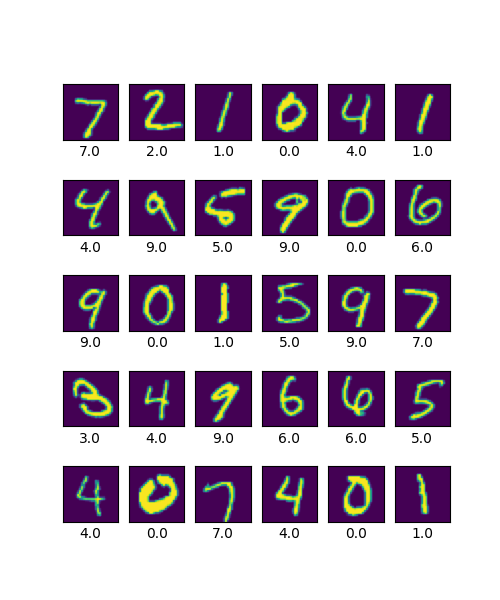
\includegraphics[width=\linewidth]{dataset_mnist.png}
    $ZT1$
\endminipage\hfill
\minipage{0.32\textwidth}
    \centering
    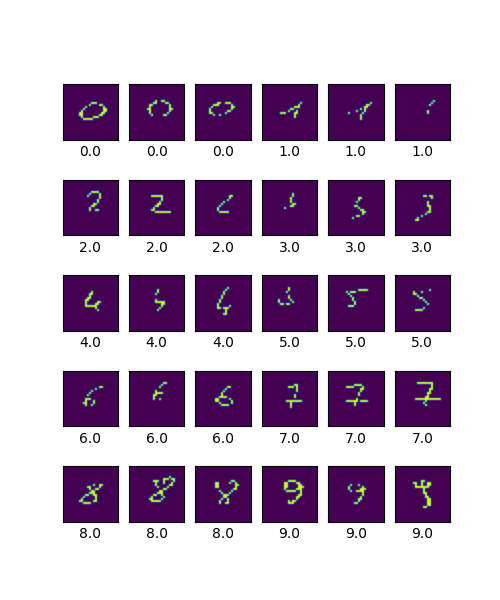
\includegraphics[width=\linewidth]{dataset_my.png}
    $ZT2$
\endminipage\hfill
\minipage{0.32\textwidth}
    \centering
    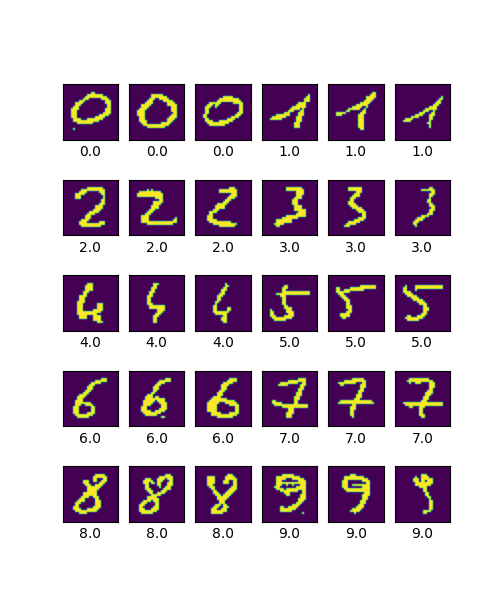
\includegraphics[width=\linewidth]{dataset_my_preprocessed.png}
    $ZT2\_PREPROCESSED$
\endminipage
\end{figure}

\section*{Wybór parametrów}
Klasteryzacja została przeprowadzona wykonując 50 iteracji dla każdego testu, oraz po 5 testów na przypadek. Następnie wybierana była najlepsza klasteryzacja (o najniższej inercji)

\section*{Porównanie macierzy dopasowania}
\phantom{.}\\
\begin{tabular}{ |c|c|c|c|c|c|c| }
    \hline
        k & $ZT$ & $ZT1$ & $ZT2$ & $ZT2\_PRE$ & $ZT3$ & $ZT3\_PRE$ \\
    \hline
        7 & 
        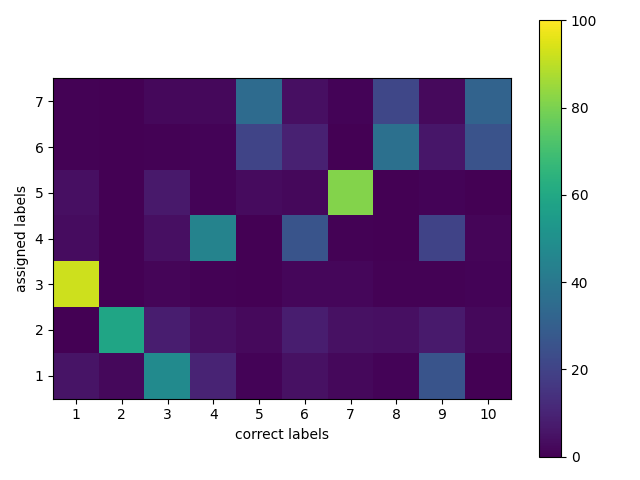
\includegraphics[width=0.13\linewidth]{../results/7-clusters/accuracy - train.png} &
        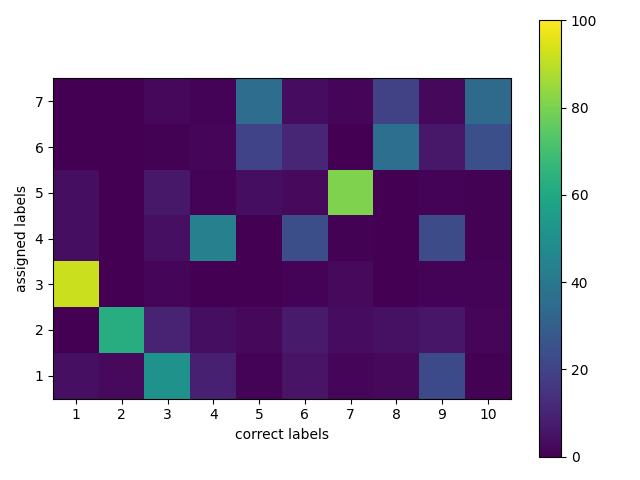
\includegraphics[width=0.13\linewidth]{../results/7-clusters/accuracy - test 1.png} &
        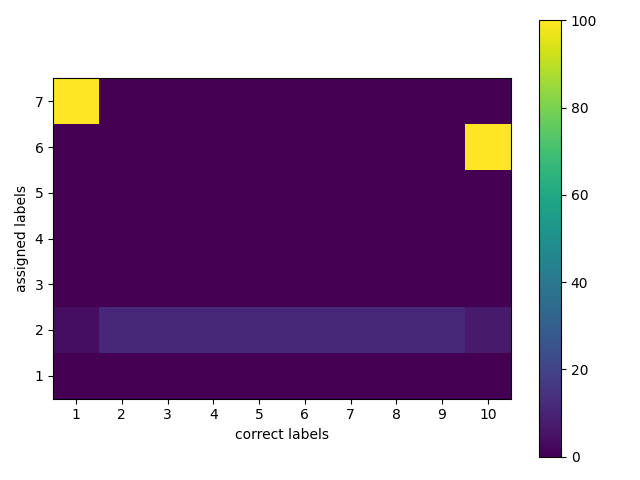
\includegraphics[width=0.13\linewidth]{../results/7-clusters/accuracy - test 2.png} &
        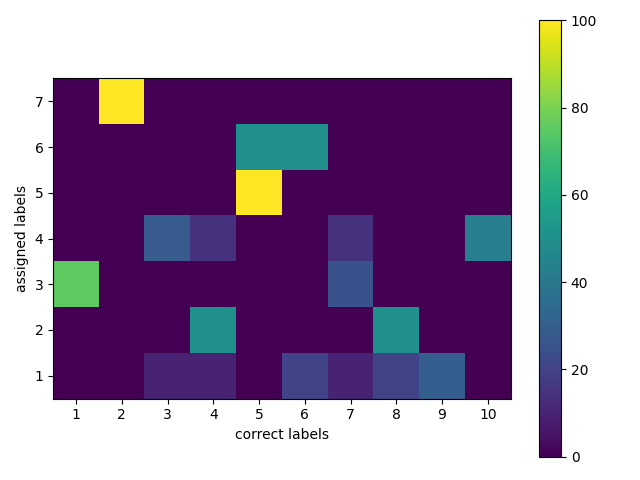
\includegraphics[width=0.13\linewidth]{../results/7-clusters/accuracy - test 2 preprocessed.png} &
        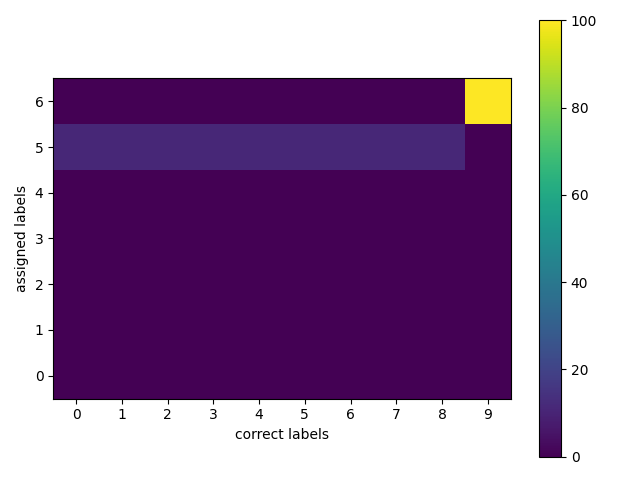
\includegraphics[width=0.13\linewidth]{../results/7-clusters/accuracy - test 3.png} &
        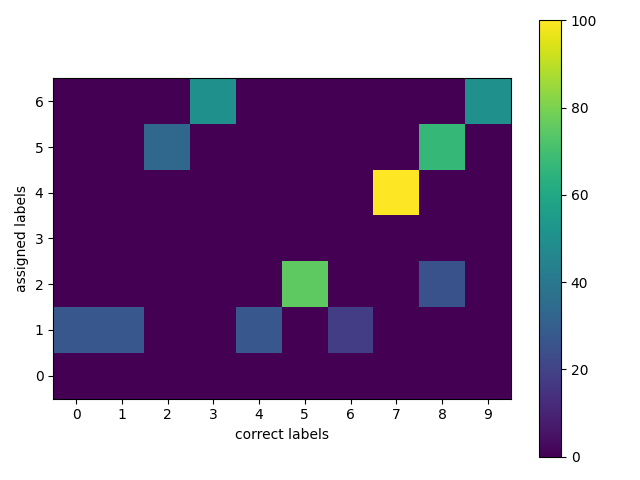
\includegraphics[width=0.13\linewidth]{../results/7-clusters/accuracy - test 3 preprocessed.png} \\
    \hline
        8 & 
        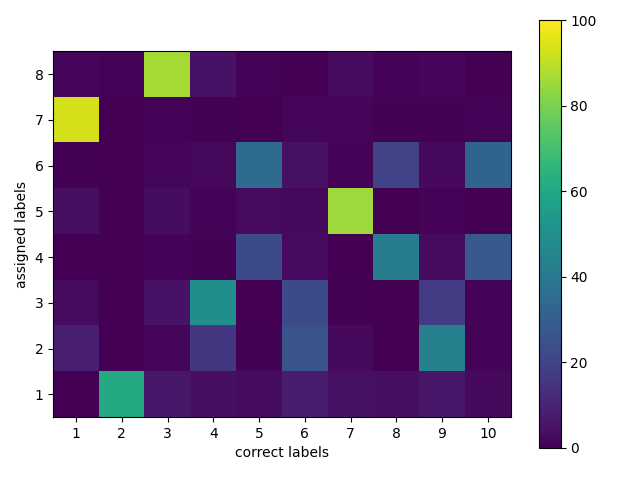
\includegraphics[width=0.13\linewidth]{../results/8-clusters/accuracy - train.png} &
        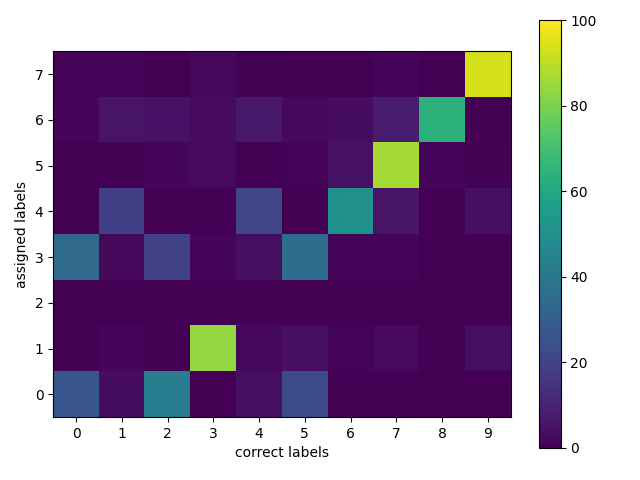
\includegraphics[width=0.13\linewidth]{../results/8-clusters/accuracy - test 1.png} &
        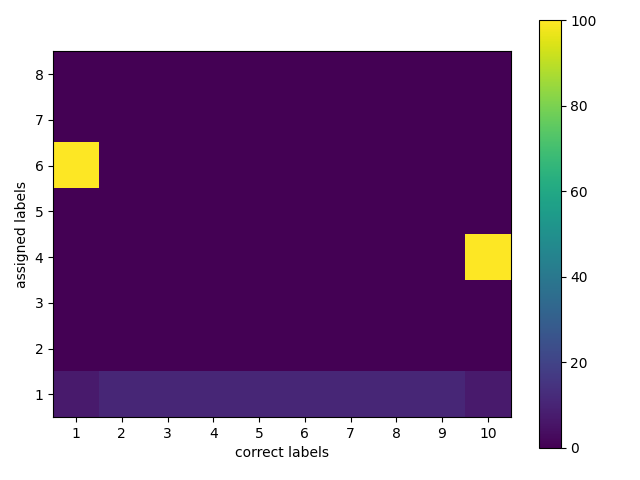
\includegraphics[width=0.13\linewidth]{../results/8-clusters/accuracy - test 2.png} &
        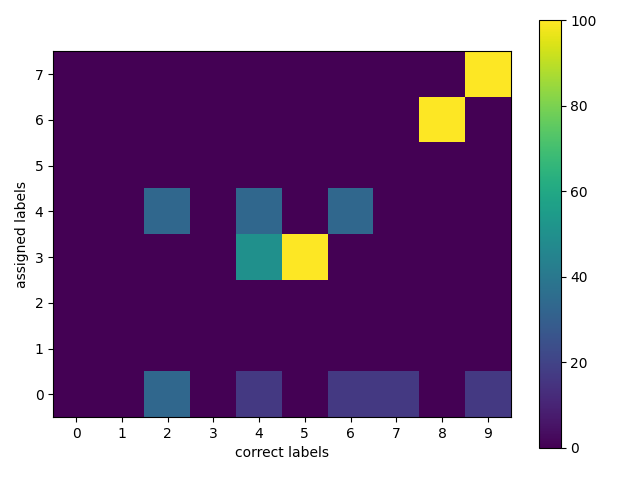
\includegraphics[width=0.13\linewidth]{../results/8-clusters/accuracy - test 2 preprocessed.png} &
        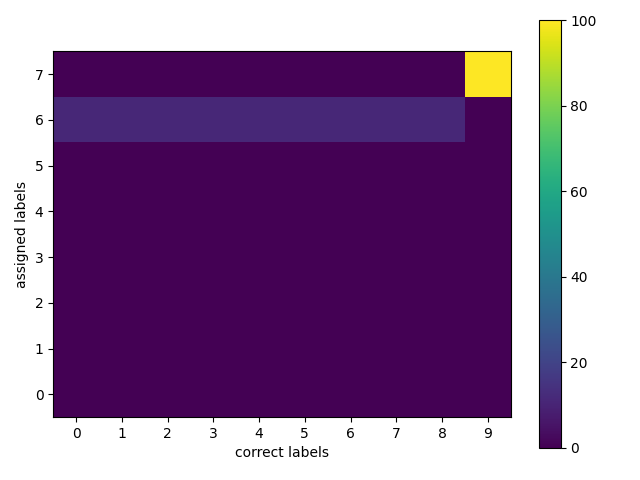
\includegraphics[width=0.13\linewidth]{../results/8-clusters/accuracy - test 3.png} &
        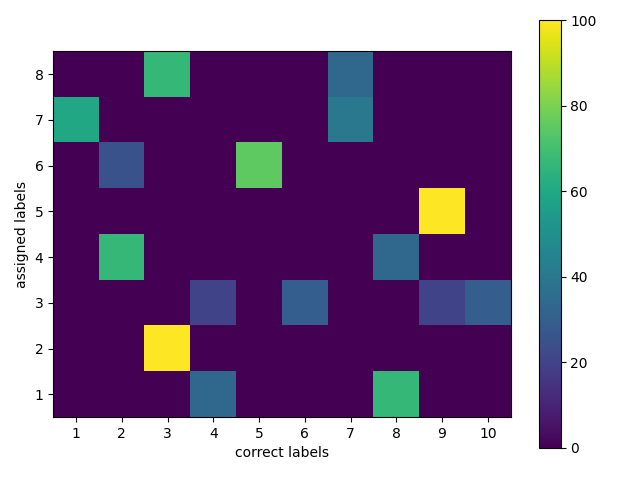
\includegraphics[width=0.13\linewidth]{../results/8-clusters/accuracy - test 3 preprocessed.png} \\
    \hline
        9 & 
        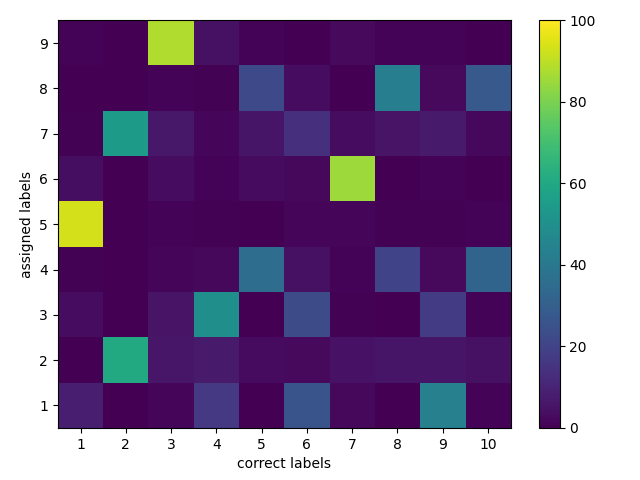
\includegraphics[width=0.13\linewidth]{../results/9-clusters/accuracy - train.png} &
        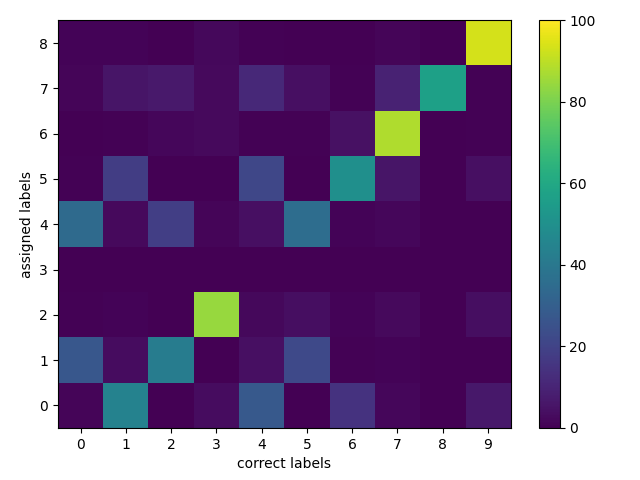
\includegraphics[width=0.13\linewidth]{../results/9-clusters/accuracy - test 1.png} &
        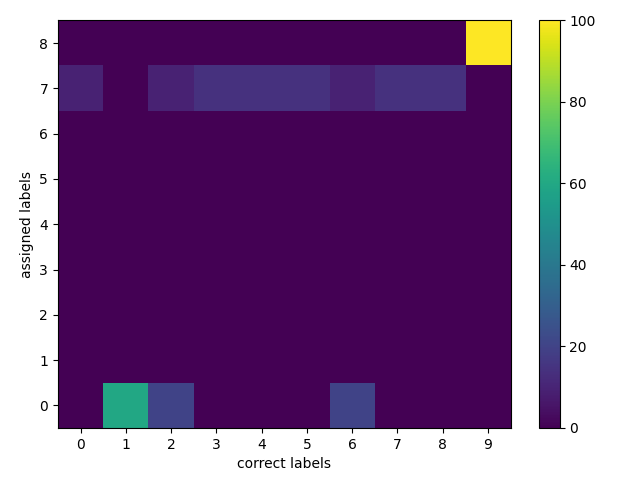
\includegraphics[width=0.13\linewidth]{../results/9-clusters/accuracy - test 2.png} &
        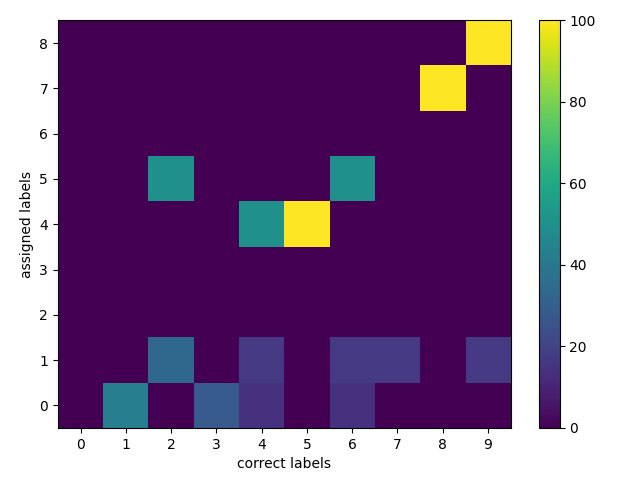
\includegraphics[width=0.13\linewidth]{../results/9-clusters/accuracy - test 2 preprocessed.png} &
        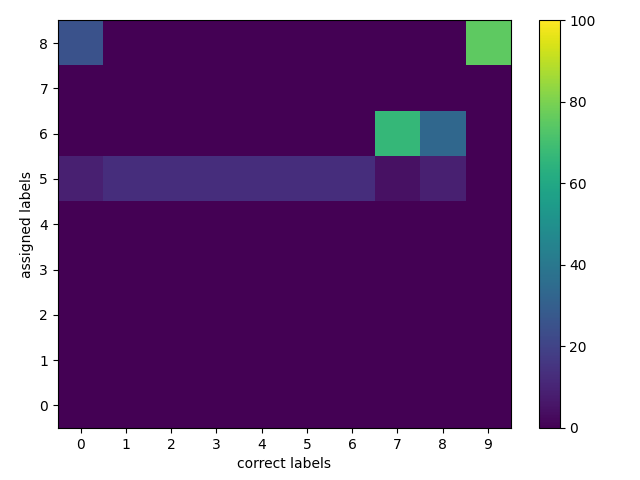
\includegraphics[width=0.13\linewidth]{../results/9-clusters/accuracy - test 3.png} &
        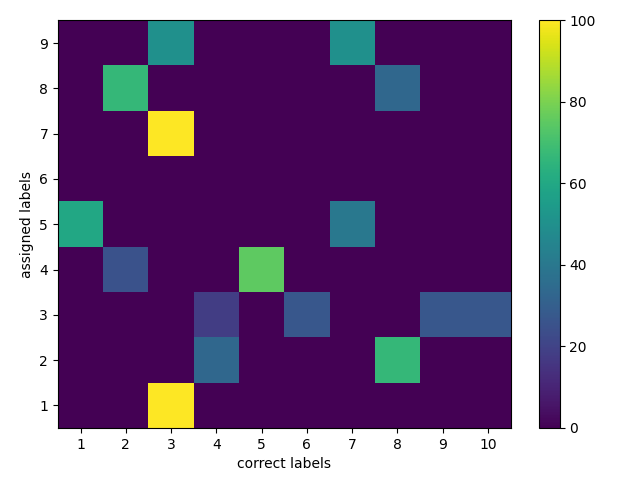
\includegraphics[width=0.13\linewidth]{../results/9-clusters/accuracy - test 3 preprocessed.png} \\
    \hline
        10 & 
        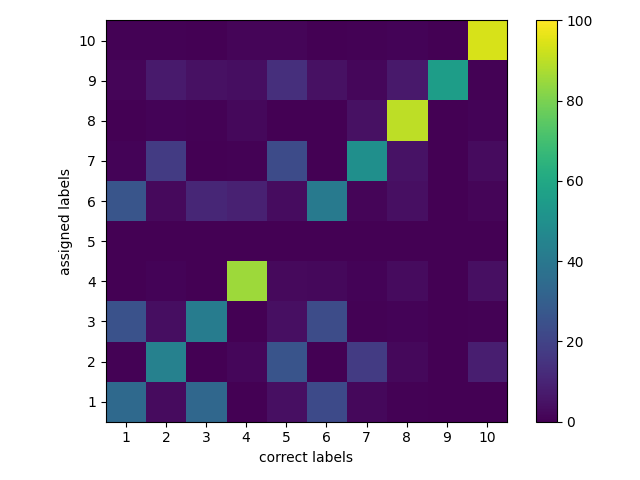
\includegraphics[width=0.13\linewidth]{../results/10-clusters/accuracy - train.png} &
        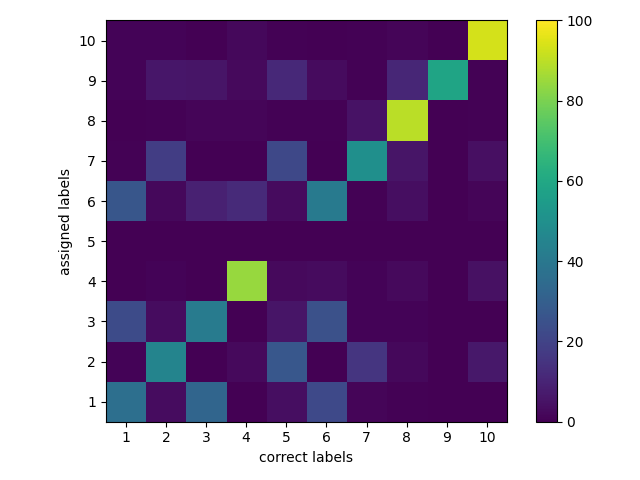
\includegraphics[width=0.13\linewidth]{../results/10-clusters/accuracy - test 1.png} &
        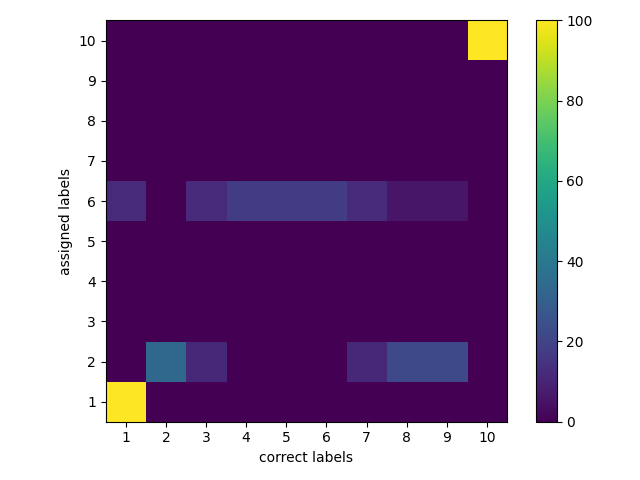
\includegraphics[width=0.13\linewidth]{../results/10-clusters/accuracy - test 2.png} &
        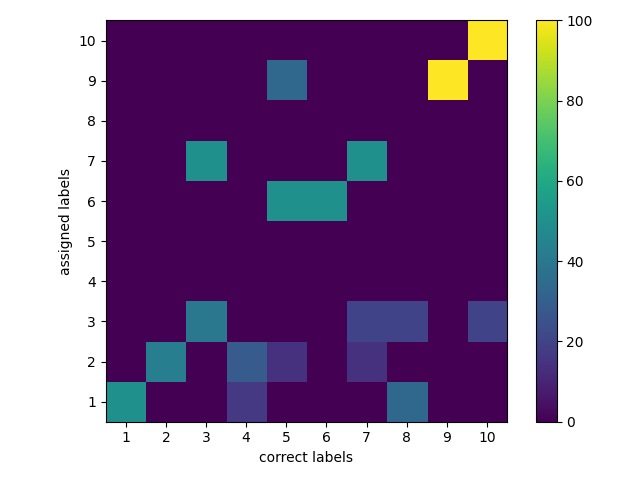
\includegraphics[width=0.13\linewidth]{../results/10-clusters/accuracy - test 2 preprocessed.png} &
        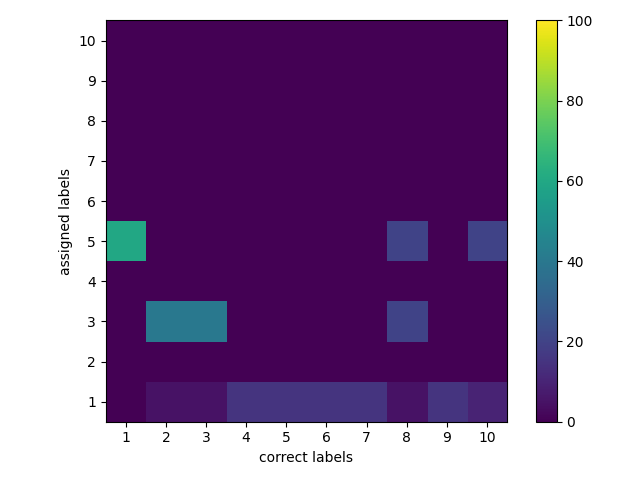
\includegraphics[width=0.13\linewidth]{../results/10-clusters/accuracy - test 3.png} &
        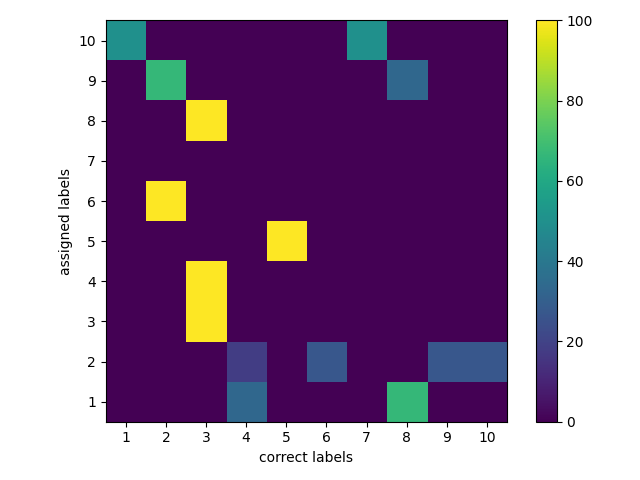
\includegraphics[width=0.13\linewidth]{../results/10-clusters/accuracy - test 3 preprocessed.png} \\
    \hline
        11 & 
        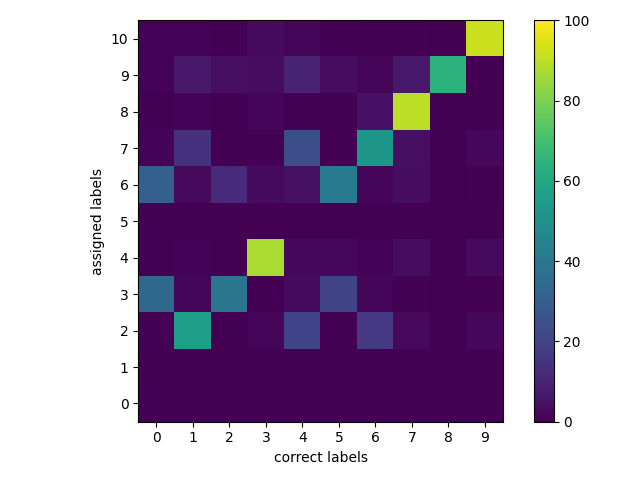
\includegraphics[width=0.13\linewidth]{../results/11-clusters/accuracy - train.png} &
        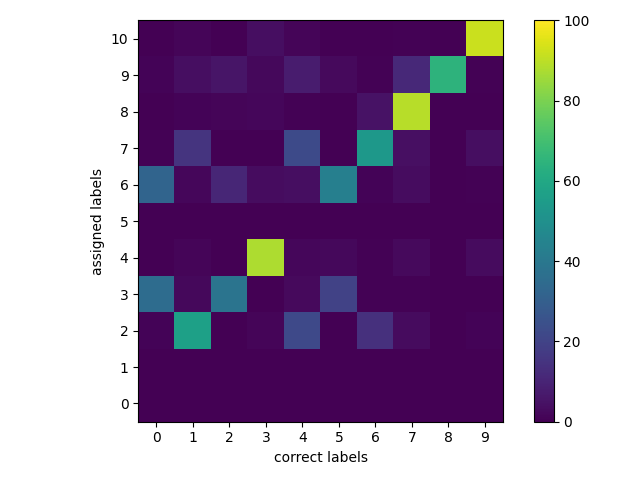
\includegraphics[width=0.13\linewidth]{../results/11-clusters/accuracy - test 1.png} &
        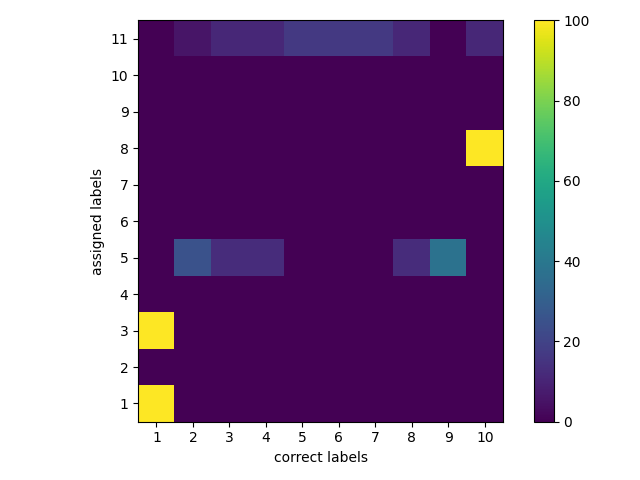
\includegraphics[width=0.13\linewidth]{../results/11-clusters/accuracy - test 2.png} &
        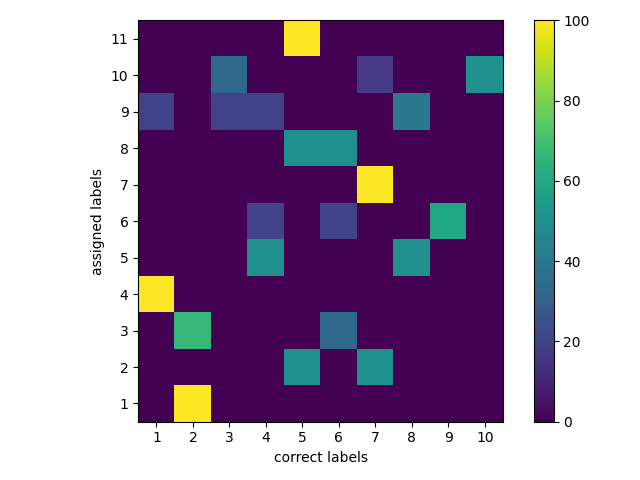
\includegraphics[width=0.13\linewidth]{../results/11-clusters/accuracy - test 2 preprocessed.png} &
        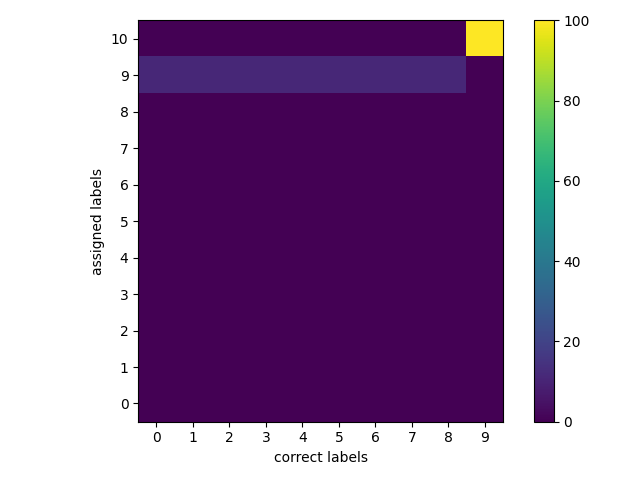
\includegraphics[width=0.13\linewidth]{../results/11-clusters/accuracy - test 3.png} &
        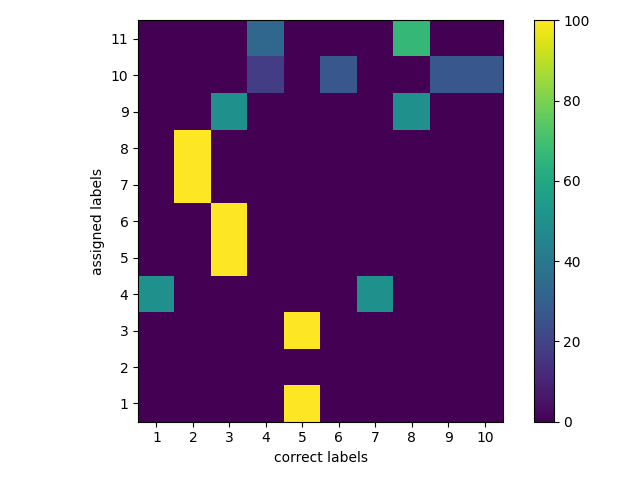
\includegraphics[width=0.13\linewidth]{../results/11-clusters/accuracy - test 3 preprocessed.png} \\
    \hline
        12 & 
        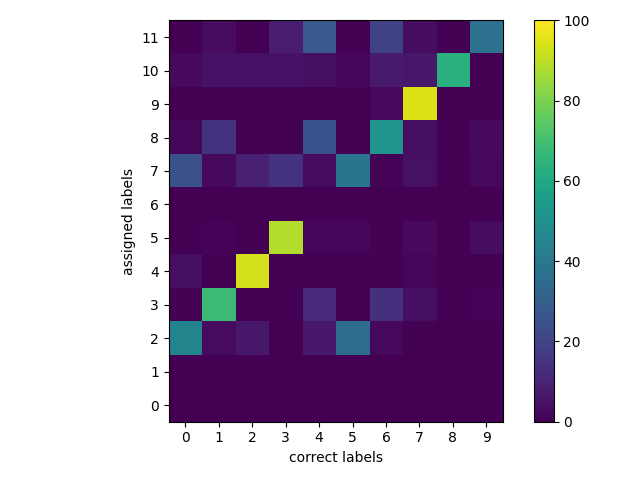
\includegraphics[width=0.13\linewidth]{../results/12-clusters/accuracy - train.png} &
        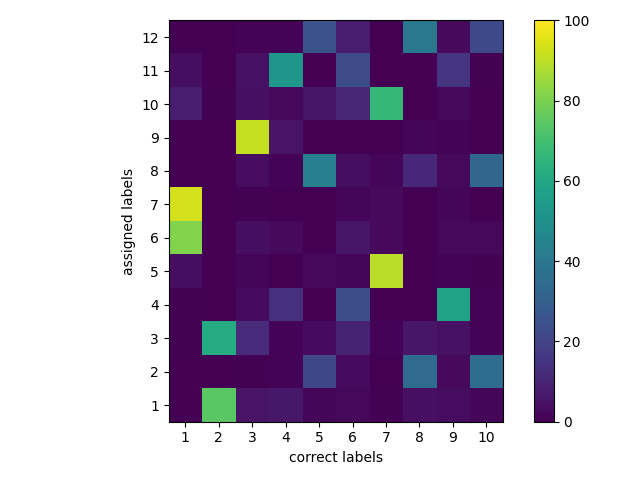
\includegraphics[width=0.13\linewidth]{../results/12-clusters/accuracy - test 1.png} &
        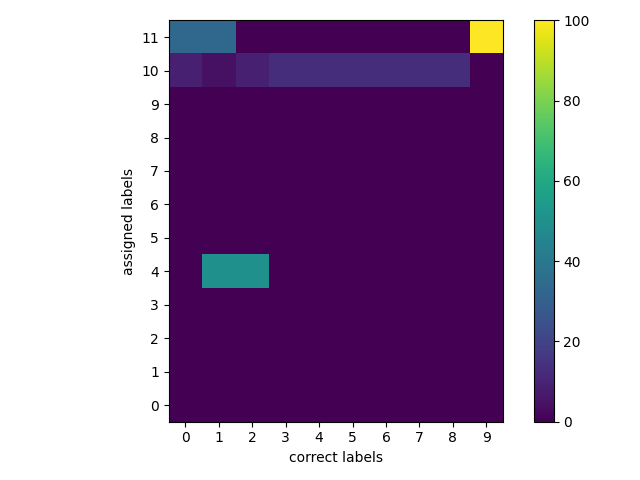
\includegraphics[width=0.13\linewidth]{../results/12-clusters/accuracy - test 2.png} &
        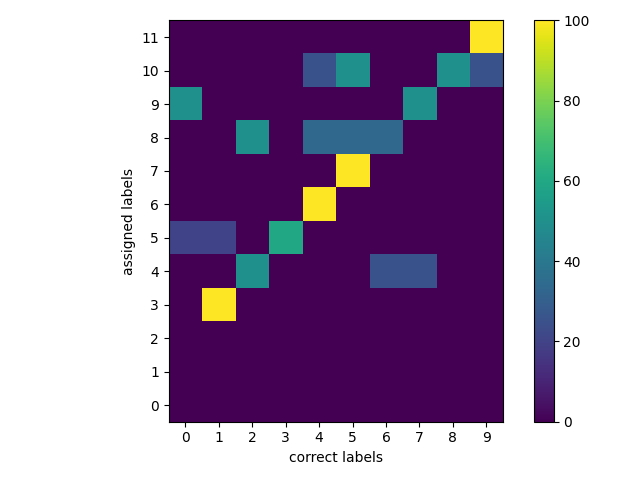
\includegraphics[width=0.13\linewidth]{../results/12-clusters/accuracy - test 2 preprocessed.png} &
        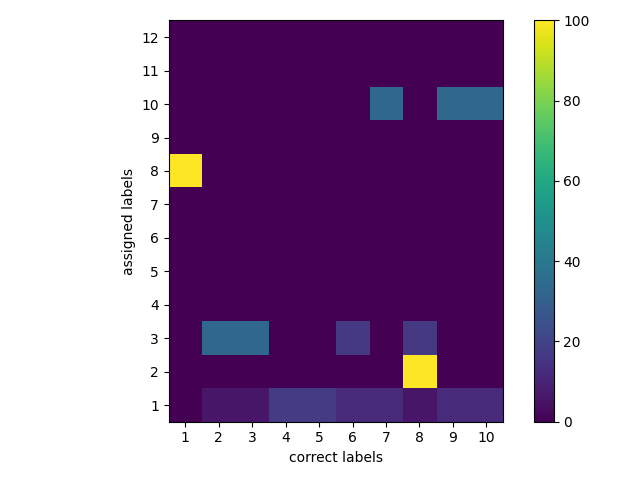
\includegraphics[width=0.13\linewidth]{../results/12-clusters/accuracy - test 3.png} &
        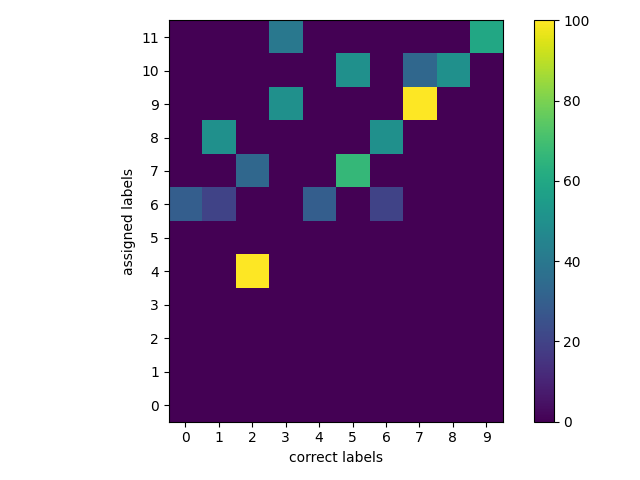
\includegraphics[width=0.13\linewidth]{../results/12-clusters/accuracy - test 3 preprocessed.png} \\
    \hline
\end{tabular}

\section*{Porównanie centroidów}
\phantom{.}\\
\begin{tabular}{ |c|c|c| }
    \hline
        k & centroidy początkowe & centroidy finalne \\
    \hline
        7 & 
        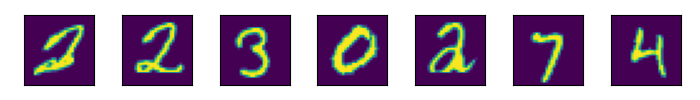
\includegraphics[width=0.45\linewidth]{../results/7-clusters/centroids_start.png} &
        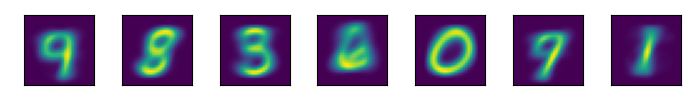
\includegraphics[width=0.45\linewidth]{../results/7-clusters/centroids_end.png} \\
    \hline
        8 & 
        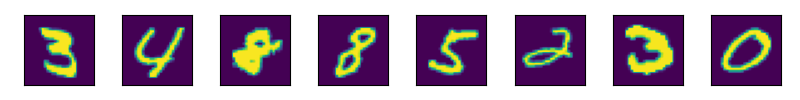
\includegraphics[width=0.45\linewidth]{../results/8-clusters/centroids_start.png} &
        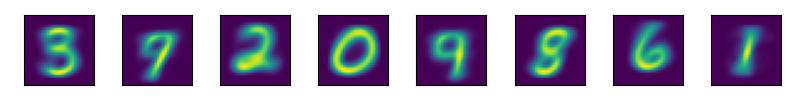
\includegraphics[width=0.45\linewidth]{../results/8-clusters/centroids_end.png} \\
    \hline
        9 & 
        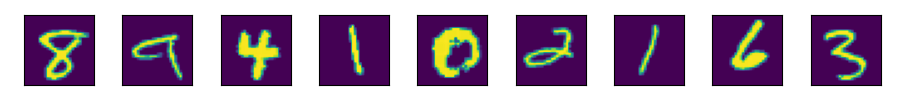
\includegraphics[width=0.45\linewidth]{../results/9-clusters/centroids_start.png} &
        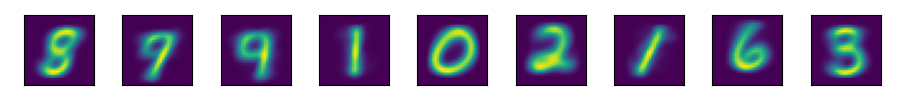
\includegraphics[width=0.45\linewidth]{../results/9-clusters/centroids_end.png} \\
    \hline
        10 & 
        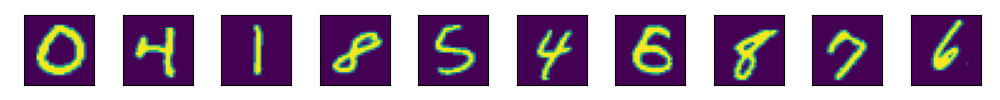
\includegraphics[width=0.45\linewidth]{../results/10-clusters/centroids_start.png} &
        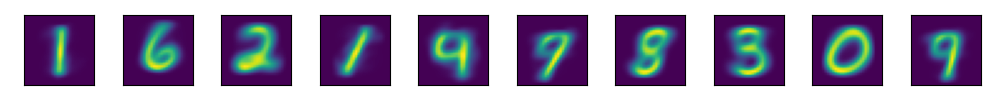
\includegraphics[width=0.45\linewidth]{../results/10-clusters/centroids_end.png} \\
    \hline
        11 & 
        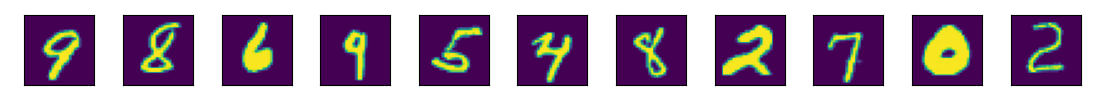
\includegraphics[width=0.45\linewidth]{../results/11-clusters/centroids_start.png} &
        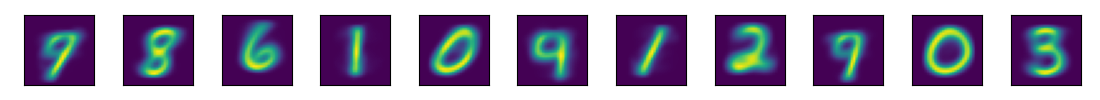
\includegraphics[width=0.45\linewidth]{../results/11-clusters/centroids_end.png} \\
    \hline
        12 & 
        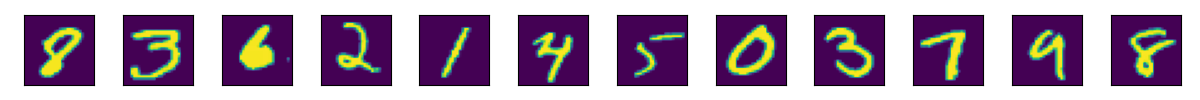
\includegraphics[width=0.45\linewidth]{../results/12-clusters/centroids_start.png} &
        \includegraphics[width=0.45\linewidth]{../results/12-clusters/centroids_end.png} \\
    \hline
\end{tabular}

\vspace{2cm}

\section*{Porównanie inercji}
Inercja malała wraz ze wzrostem ilości klastrów.\\

\begin{center}
    \begin{tikzpicture}
        \begin{axis}[xlabel=\(klastry\), ylabel=\(inercja\)]
            \addplot[color=red, mark=square]coordinates{
                (7,451.88357820613015)
                (8,387.8188056476413)
                (9,338.55770390981905)
                (10,300.1596545283836)
                (11,268.8125225761924)
                (12,243.61689830482396)};
        \end{axis}
    \end{tikzpicture}
\end{center}
